
%(BEGIN_QUESTION)
% Copyright 2013, Tony R. Kuphaldt, released under the Creative Commons Attribution License (v 1.0)
% This means you may do almost anything with this work of mine, so long as you give me proper credit

Suppose a long length of multi-pair instrument cable is suspected of exhibiting {\it crosstalk}, where current traveling through one wire pair magnetically induces electrical noise on an adjacent wire pair.  The cable has been removed from service and is wrapped up on a spool awaiting testing.  Looking at one end of this cable, you see this:

$$\includegraphics[width=15.5cm]{i03545x01.eps}$$

Devise a test by which you could prove or disprove this kind of ``crosstalk'' in the cable.  Feel free to sketch a diagram of the test circuit if you find that helpful.

\underbar{file i03545}
%(END_QUESTION)





%(BEGIN_ANSWER)

Connect two jumper wires to the other end of the cable: one jumper wire shorting together the red and black conductors of pair 1, and the other jumper wires doing the same for pair 2.  Now, connect an AC signal source to the other end of pair 1, in order to generate an AC current through that wire pair.  Connect an AC voltmeter to the other end of pair 2, in order to measure any induced voltage.  If you detect AC voltage induced in pair 2, you know there is crosstalk between pairs 1 and 2. 

\vskip 10pt

Failing to jumper the pairs at the cable's far end is worth only half-credit, because without a complete loop there would be no electric current and therefore no magnetic field generated.

\vskip 10pt

Using DC instead of AC is also worth only half-credit.

%(END_ANSWER)





%(BEGIN_NOTES)

{\bf This question is intended for exams only and not worksheets!}.

%(END_NOTES)


